\documentclass[12pt]{article}

\usepackage{mathpazo}
\usepackage{amsmath}
\usepackage{graphicx}
\usepackage{booktabs}
\usepackage{listings}
\usepackage{xcolor}
\usepackage{array}
\usepackage{geometry}
\usepackage{float}
\pagestyle{empty}
\geometry{margin=1in}

\lstset{
    basicstyle=\ttfamily\small,
    breaklines=true,
    frame=single,
    backgroundcolor=\color{gray!10}
}

\title{\textbf{Regression Analysis Assignment}}
\date{}

\begin{document}

\maketitle

\section{Dataset Selection}

The California Housing Dataset was selected for this regression task. It is available through the Scikit-learn library and represents a real-world problem of predicting housing prices.

\subsection*{Dataset Overview}

\begin{center}
\renewcommand{\arraystretch}{1.5}
\setlength{\tabcolsep}{10pt}
\begin{tabular}{|m{5cm}|m{8cm}|}
\hline
\textbf{Attribute} & \textbf{Description} \\
\hline
Source & Scikit-learn dataset repository \\
\hline
Features & Income, house age, rooms, bedrooms, population, occupancy, latitude, longitude \\
\hline
Target & Median house value \\
\hline
Total Rows & 20,640 \\
\hline
\end{tabular}
\end{center}

\subsection{Sample Data Instances}

\begin{center}
\renewcommand{\arraystretch}{1.6}
\setlength{\tabcolsep}{2.8pt}
\begin{tabular}{|c|c|c|c|c|c|c|c|c|c|}
\hline
\textbf{Index} & \textbf{MedInc} & \textbf{HouseAge} & \textbf{AveRooms} & \textbf{AveBedrms} & \textbf{Population} & \textbf{AveOccup} & \textbf{Lat} & \textbf{Long} & \textbf{Target} \\
\hline
0 & 8.3252 & 41 & 6.98 & 1.02 & 322 & 2.56 & 37.88 & -122.23 & 4.526 \\
\hline
1 & 8.3014 & 21 & 6.24 & 0.97 & 2401 & 2.11 & 37.86 & -122.22 & 3.585 \\
\hline
2 & 7.2574 & 52 & 8.29 & 1.07 & 496 & 2.80 & 37.85 & -122.24 & 3.521 \\
\hline
3 & 5.6431 & 52 & 5.82 & 1.07 & 558 & 2.55 & 37.85 & -122.25 & 3.413 \\
\hline
4 & 3.8462 & 52 & 6.28 & 1.08 & 565 & 2.18 & 37.85 & -122.25 & 3.422 \\
\hline
\end{tabular}
\end{center}

\textbf{Explanation:}  
The table presents sample records from the dataset, showing how input features and the target variable are structured. It helps in understanding data variation and feature ranges.

\section{Dataset Visualization}

\subsection{Feature Distribution}

\begin{figure}[H]
\centering
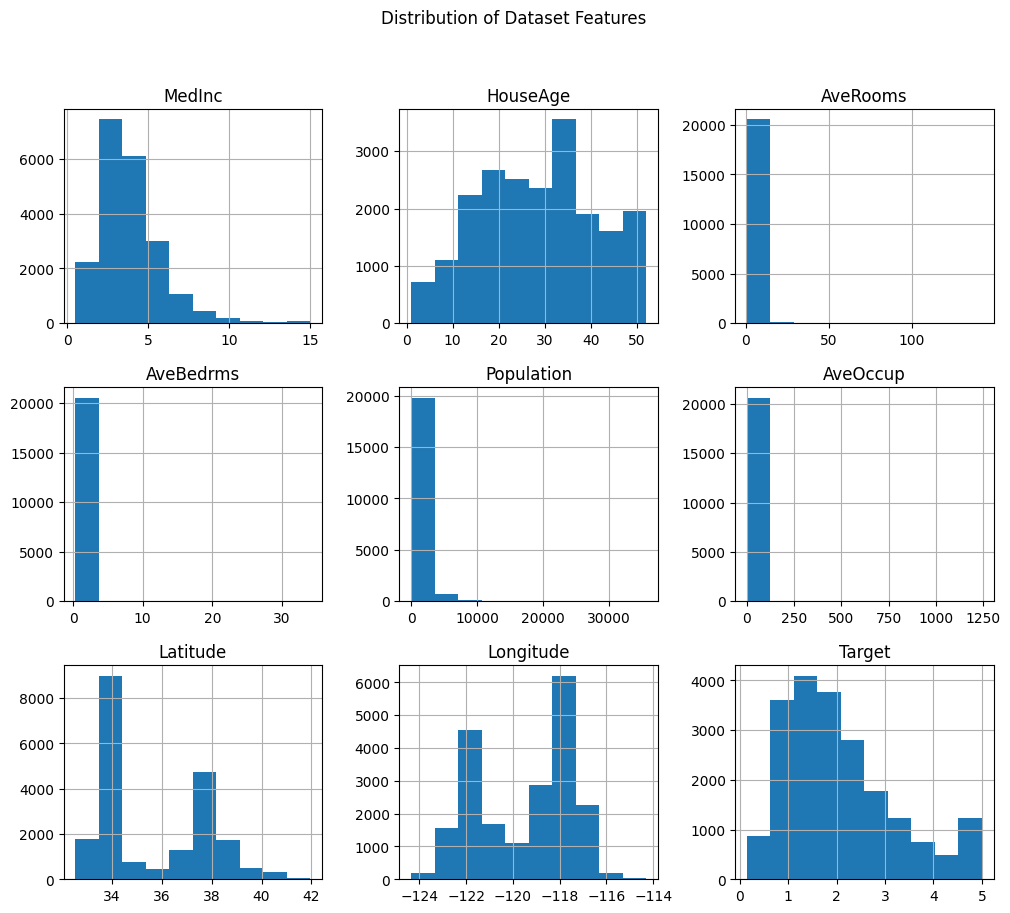
\includegraphics[width=1.0\textwidth]{feature_distribution.png}
\caption{Distribution of Dataset Features}
\end{figure}

\textbf{Explanation:}  
The histogram shows the distribution of all features, highlighting differences in scale and skewness. This justifies preprocessing steps such as feature scaling.

\section{Data Preprocessing}

\subsection{Missing Values}
No missing values were found.

\subsection{Feature Scaling}
StandardScaler was applied.

\textbf{Reason:}  
Scaling ensures all features contribute equally and improves Linear Regression performance.

\subsection{Train-Test Split}
80\% training and 20\% testing split ensures fair evaluation.

\section{Model Implementation}

\subsection{Code}

\begin{lstlisting}[language=Python]
from sklearn.datasets import fetch_california_housing
from sklearn.model_selection import train_test_split
from sklearn.preprocessing import StandardScaler
from sklearn.linear_model import LinearRegression
from sklearn.ensemble import RandomForestRegressor

data = fetch_california_housing()
X, y = data.data, data.target

X_train, X_test, y_train, y_test = train_test_split(
    X, y, test_size=0.2, random_state=42)

scaler = StandardScaler()
X_train_scaled = scaler.fit_transform(X_train)
X_test_scaled = scaler.transform(X_test)

lr = LinearRegression()
rf = RandomForestRegressor(n_estimators=100, random_state=42)

lr.fit(X_train_scaled, y_train)
rf.fit(X_train, y_train)

y_pred_lr = lr.predict(X_test_scaled)
y_pred_rf = rf.predict(X_test)
\end{lstlisting}

\textbf{Explanation:}  
The dataset is loaded and split into training and testing sets. Feature scaling is applied for Linear Regression. Two models are trained: Linear Regression (linear model) and Random Forest (ensemble model). Predictions are generated using both models.

\section{Model Evaluation}

\begin{lstlisting}[language=Python]
from sklearn.metrics import mean_absolute_error, mean_squared_error, r2_score
import numpy as np

def evaluate(y_test, y_pred):
    mae = mean_absolute_error(y_test, y_pred)
    mse = mean_squared_error(y_test, y_pred)
    rmse = np.sqrt(mse)
    r2 = r2_score(y_test, y_pred)
    return mae, mse, rmse, r2
\end{lstlisting}

\textbf{Explanation:}  
This function computes evaluation metrics including MAE, MSE, RMSE, and $R^2$, which measure prediction error and model performance.

\subsection{Results}

\begin{center}
\renewcommand{\arraystretch}{1.6}
\setlength{\tabcolsep}{12pt}
\begin{tabular}{|c|c|c|c|c|}
\hline
\textbf{Model} & \textbf{MAE} & \textbf{MSE} & \textbf{RMSE} & \textbf{$R^2$} \\
\hline
Linear Regression & 0.53 & 0.55 & 0.74 & 0.58 \\
\hline
Random Forest & 0.33 & 0.25 & 0.50 & 0.81 \\
\hline
\end{tabular}
\end{center}

\textbf{Analysis:}  
Random Forest shows lower errors and higher $R^2$, indicating better predictive performance.

\section{Visualization and Analysis}

\subsection{Actual vs Predicted Values}

\begin{figure}[H]
\centering
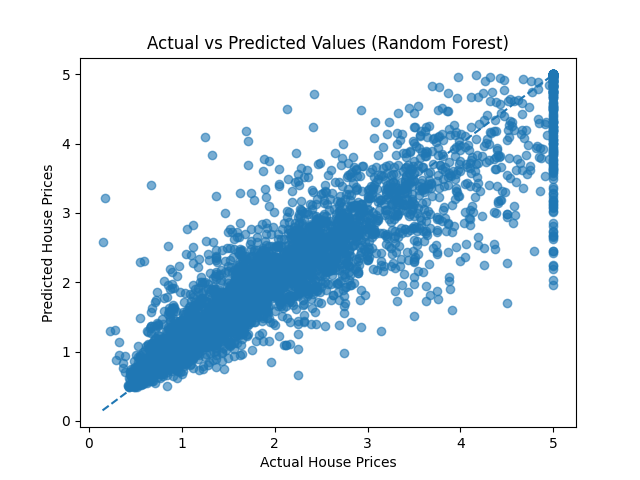
\includegraphics[width=1.0\textwidth]{actual_vs_predicted.png}
\caption{Actual vs Predicted House Prices}
\end{figure}

\textbf{Explanation:}  
Points close to the diagonal indicate accurate predictions. The model captures the overall trend effectively.

\subsection{Actual vs Predicted (Line Comparison)}

\begin{figure}[H]
\centering
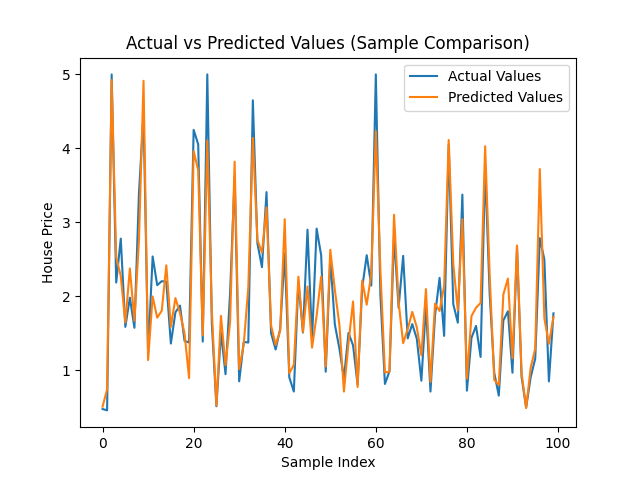
\includegraphics[width=1.0\textwidth]{line_comparison.png}
\caption{Actual vs Predicted Comparison}
\end{figure}

\textbf{Explanation:}  
Predicted values closely follow actual values, showing consistent performance.

\subsection{Feature Importance}

\begin{figure}[H]
\centering
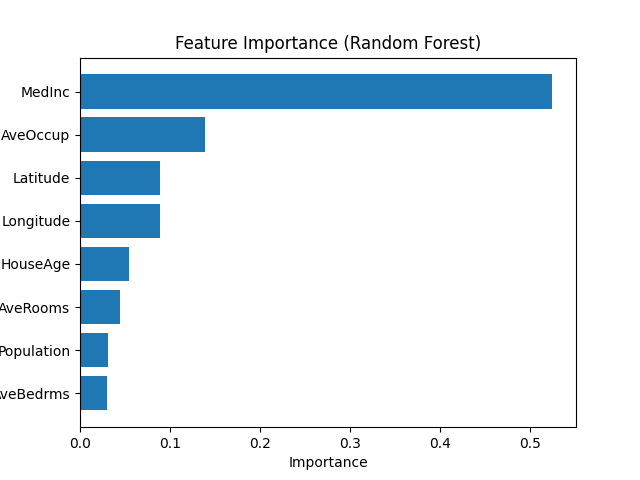
\includegraphics[width=1.0\textwidth]{feature_importance.png}
\caption{Feature Importance}
\end{figure}

\textbf{Explanation:}  
Median income has the highest importance, indicating strong influence on house prices.

\section{Final Model Justification}

Random Forest Regression is selected as the best-performing model.

\begin{itemize}
    \item Captures non-linear relationships
    \item Handles feature interactions
    \item Provides higher accuracy
\end{itemize}

\section{Conclusion}

The report demonstrates a complete regression analysis workflow. Random Forest outperforms Linear Regression due to its ability to model complex patterns and provide more accurate predictions.

\end{document}